% ----------------------------------------------------------------------
% Template VERIFICA
% ----------------------------------------------------------------------
% 2020 di d!egofantinelli at jazzmagus@gmail.com
% ----------------------------------------------------------------------

% ---------------------------------- Preambolo
\documentclass[11pt, a4paper]{exam}
\usepackage[T1]{fontenc}
\usepackage{mdframed}
%\usepackage{nicefrac}
%\usepackage[applemac]{inputenc}
%\usepackage[utf8]{inputenc}
\usepackage[italian]{babel}
\usepackage[margin=1.3in]{geometry}
\usepackage{amsmath,amssymb}
\usepackage{multicol}
\usepackage{graphicx}
\usepackage{tikz}
\usepackage{upquote}
\usepackage{caption}
\usepackage{enumitem}
\usepackage{float}

\printanswers

% ---------------------------------- Command
\renewcommand{\questionshook}{%
    \setlength{\leftmargin}{0pt}%
}
\renewcommand{\choiceshook}{%
    \setlength{\leftmargin}{20pt}%
}

\newcommand{\class}{\huge {Verifica di Matematica}}
\newcommand{\term}{02 | 02}
\newcommand{\examnum}{Verifica numero: 02/02}
\newcommand{\examdate}{06 maggio 2021}
\newcommand{\timelimit}{50 minuti}

\CorrectChoiceEmphasis{\color{red}}
\SolutionEmphasis{\color{red} \footnotesize}
\renewcommand{\solutiontitle}{\noindent\textbf{Soluzione:}\par\noindent}

% ---------------------------------- Headers and Footers

\pagestyle{headandfoot}
\firstpageheader{IIS "G.A. Remondini" - Bassano del Grappa (VI)}{}{\examdate}
\runningheader{\footnotesize VERIFICA di MATEMATICA}{}{Classe 5\string^QAz}
\runningheadrule

\firstpagefooter{}{}{pag. \thepage\ di \numpages}
\runningfooter{}{}{pag. \thepage\ di \numpages}
\runningfootrule

% ---------------------------------- Punteggi
\pointpoints{punto}{\em punti}
\pointformat{[{\footnotesize \thepoints}]}
\bonuspointpoints{punto bonus}{\em punti bonus}
\bonuspointformat{[{\footnotesize \thepoints}]}
\pointsinrightmargin
\setlength{\rightpointsmargin}{.2cm}
\chqword{Esercizio}
\chpword{Punti}
\chbpword{Punti Bonus}
\chsword{Punteggio}
\chtword{Totale}

\begin{document}

% ---------------------------------- Title Page
\begin{center}
\rule[2ex]{\textwidth}{0.5pt}\\
{\huge{\bf \class}}\\[12pt]
{\huge \examnum}\\[8pt]
\rule[2ex]{\textwidth}{0.5pt}\\
\end{center}
\vspace{3cm}
\begin{tabular*}{\textwidth}{l @{\extracolsep{\fill}} r @{\extracolsep{6pt}} l}
\textbf{} & \textbf{Cognome e Nome:} & \makebox[2.5in]{\hrulefill}\\
\textbf{} &&\\
\textbf{} & \textbf{Classe:} & \makebox[2.5in]{\Large{\bf 5 \string^ QAz}}\\
\textbf{} &&\\
\textbf{} & Tempo a disposizione: & \makebox[2.5in]{\timelimit}
\end{tabular*}\\[3cm]
\vspace{5cm}
% ---------------------------------- Avvertenze

\noindent
\rule[2ex]{\textwidth}{0.2pt}
\textbf{Avvertenze}:
\begin{itemize}
	\item La presente Verifica - che viene somministrata in modalit� \emph{in presenza} al - contiene \numquestions \; quesiti, per un totale di \numpoints \;punti.
	\item Per gli eventuali studenti presenti in modalit� DDI la webcam dovr� rimanere accesa per tutto il tempo della verifica (\timelimit), salvo impossibilit� concrete di connessione; il microfono rester� spento e verr� acceso soltanto per chiarimenti e domande, che saranno consentite negli ultimi 20 min della prova.
	\item E' vietato l'utilizzo di calcolatrici scientifiche, smartphone, tablet e altri dispositivi digitali, nonch� la consultazione di testi, appunti e siti web.

\end{itemize}
\vspace{10pt}
\rule[2ex]{\textwidth}{0.2pt}
\vfill
\newpage

% ---------------------------------- Esercizio 1

\begin{questions}

\addpoints
\question[12]
Calcolare i seguenti limiti di Funzioni Reali:\\
Quali considerazioni puoi trarre dalle soluzioni ottenute?:

\begin{multicols}{2}
\begin{parts}
\part
\[\lim_{x \to + \infty}{\dfrac{2x^2 + 5x - 3}{x^2 +x -3}}\]
\fillwithlines{0.5in}
{\footnotesize
\begin{solution}
	\([\; 2 \;]\)
\end{solution}
}
\vspace{.5cm}

\part
\[\lim_{x \to 1} \dfrac{x^2 + x -1}{x - 1}\]\\
\fillwithlines{0.5in}
{\footnotesize
\begin{solution}
	\([\; 3 \;]\)
\end{solution}
}
\vspace{.5cm}

%\part
%\[\lim_{x \to -3} \dfrac{2x^2 + 5x -3}{x^2 - x - 6}\]\\
%\fillwithlines{0.5in}
%{\footnotesize
%\begin{solution}
%	\([\; \frac{7}{5} \;]\)
%\end{solution}
%}
%\vspace{.5cm}

\end{parts}
\end{multicols}
%\vspace{.5cm}

%------------------------------------------- Esercizio 2
\addpoints
\question [6] Data la seguente funzione: 

\[y = f(x) = \dfrac{3x^3 + 4x^2 + x -1}{x^4}\] \\
Determina:
 
\begin{enumerate}[label=(\alph*)]
	\item i limiti agli estremi dell'Insieme di Definizione
	\item le equazioni degli eventuali asintoti
\end{enumerate}  
\fillwithlines{0.75in}

\vspace{.4cm}

%------------------------------------------- Esercizio 3
\addpoints
\question [4] Quali delle seguenti affermazioni sono VERE:\\

\begin{choices}
\setlength{\leftmargin}{0pt}
 \choice Una funzione reale di variabile reale � continua se � possibile disegnarne il Grafico 
 \CorrectChoice Una funzione reale di variabile reale � sempre continua all'interno del suo Insieme di definizione
 \choice soltanto se sono presenti asintoti verticali
 \CorrectChoice Una funzione reale di variabile reale � continua in un punto $x_0$ se e solo se: 
 \[\lim_{x \to x_0}f(x) = f(x_0)\]

 \choice Una funzione reale di variabile reale � continua in un punto $x_0$ se e solo se: 
 \[\lim_{x \to x_0}f(x) = \pm \infty\]

\end{choices}
\vspace{.5cm}

\pagebreak
%------------------------------------------- Esercizio 4
\addpoints
\question[8] Il grafico riportato in Figura \ref{fig:Graf1} � relativo ad una certa funzione razionale fratta, di cui non si conosce l'espressione analitica.

\begin{enumerate}[label=(\alph*)]
	\item i limiti agli estremi dell'Insieme di Definizione
	\item le equazioni degli eventuali asintoti
\end{enumerate}  

\begin{figure}[h!]
  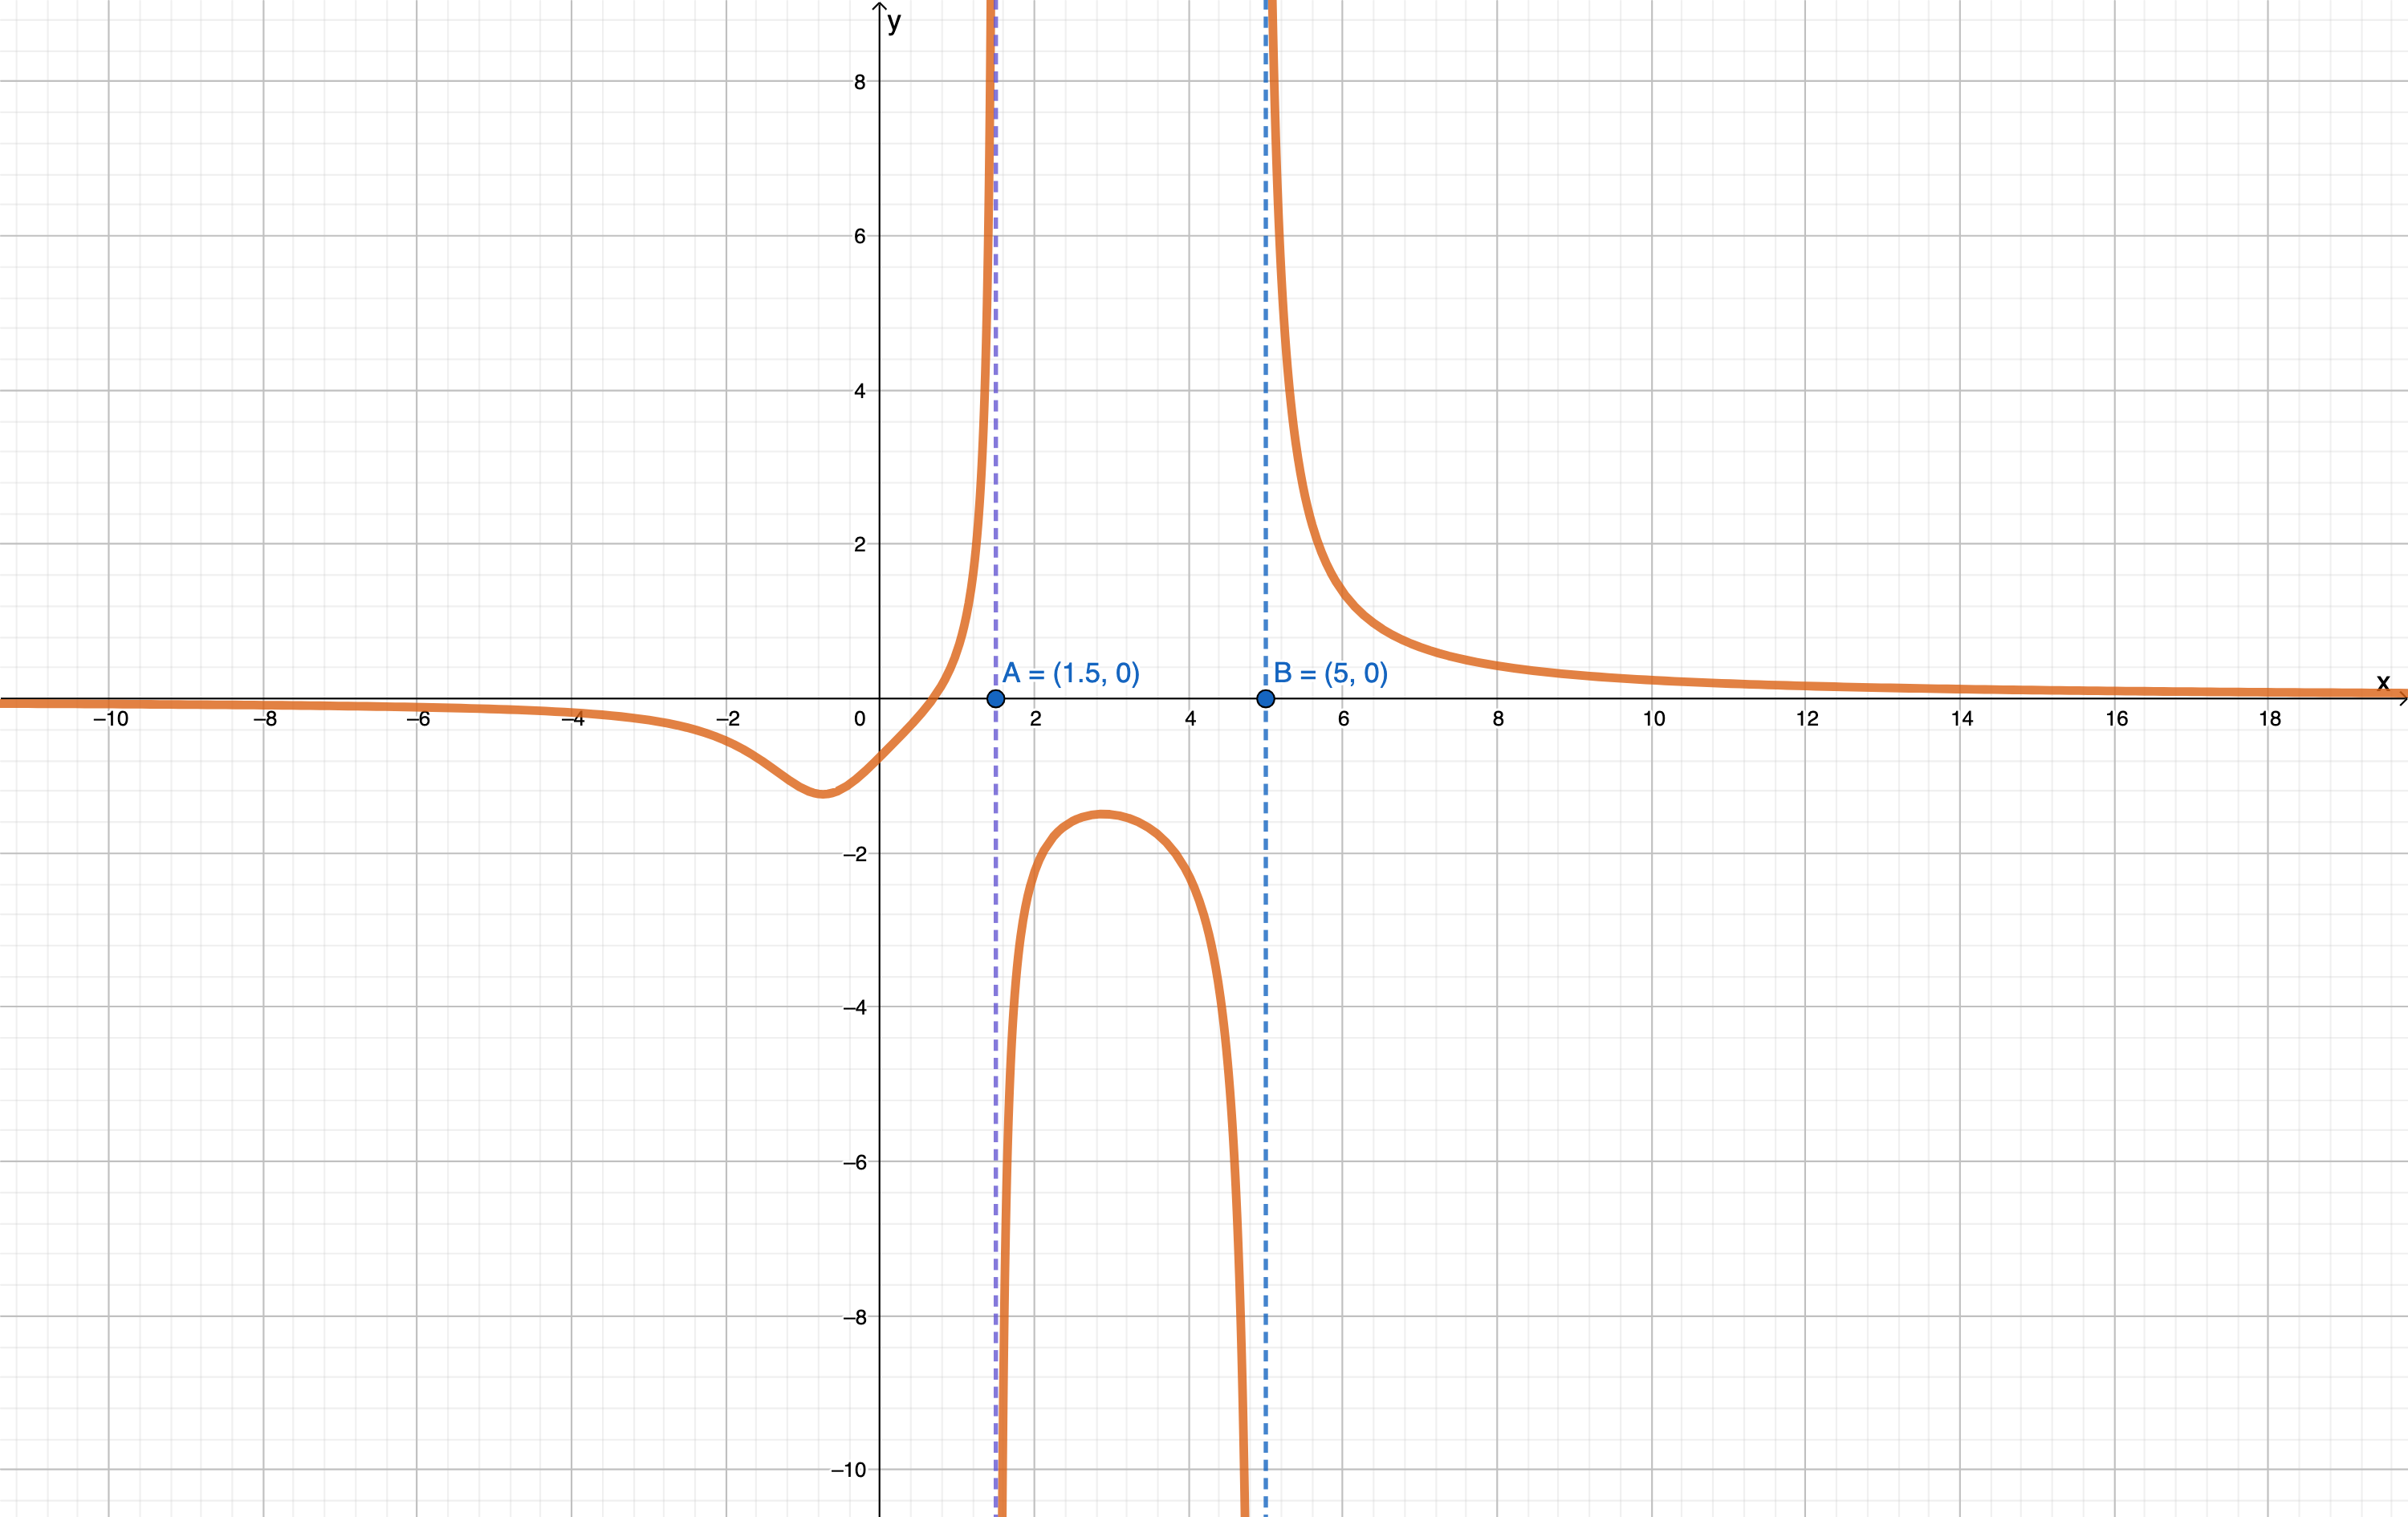
\includegraphics[width=\textwidth]{Esercizio_04}
    \caption {Grafico di una funzione razionale fratta}
\label{fig:Graf1}
\end{figure}
\fillwithlines{0.75in}

%{\footnotesize
%\begin{solution}
%	\(D = \{x \in \mathbb{R} : x \neq 1\}; \quad A(2, 0); \quad B(0, -2); \quad C(-4, 0)\)
%\end{solution}
%}
\fillwithlines{0.5in}
\end{questions}

\vfill
%\pagebreak
\noindent
\rule[2ex]{\textwidth}{1pt}

\begin{center}
{\bf Tabella dei punteggi}
\vspace{10pt}

\combinedgradetable[h][questions]
\end{center}
\vspace{10pt}
\footnotesize La sufficienza � fissata a 18 punti, ma potr� subire delle modifiche in fase di correzione, al fine di garantire la validit� della prova anche nel caso in cui si riscontrassero prestazioni della classe sensibilmente lontane dalla media-classe stimata.

\end{document}
